\chapter{BauhausBoards}\label{BauhausBoards}
Das neue Projekt bekam den Namen ``BauhausBoards''.
In einer Entwurfsphase wurde entschieden, wie das System aussehen und welche Funktionen es bieten sollte. Dabei flossen die Ergebnisse der Vorstudie und anderer Projekte mit ein.
\\
Als Voraussetzung sollten als Anzeigegeräte für die Türschilder weiterhin Tablets genutzt werden.
Der Entwurf wurde darauf in ein Programm umgesetzt, wobei manche geplanten Funktionen geändert, entfernt oder neue hinzugefügt wurden. An manchen Stellen der Umsetzung kam es auch zu Problemen, die es zu lösen galt.
% - Ergebnisse der Vorstudie sollten enbezogen werden
% - sollte weiterhin auf Tablets als Anzeigegerät laufen
% - das was im Entwurf geplant wurde musste umgesetzt werden
% - dadurch entstanden Features
% - Während der Umsetzung traten diverse Probleme auf

\section{Entwurf}\label{Entwurf}
\subsection{Entwurf des Systems}\label{Entwurf des Systems}
Die Planung des Systems begann damit, die Plattform des Systems auszuwählen.
Es gab die Möglichkeit eine Android-Applikation zu erstellen, die auf jedem Tablet hätte installiert werden müssen.
Dabei gab es jedoch das Problem, dass die Nutzer auch von unterwegs mit der Anwendung interagieren sollten, wofür ein eigenständiger Server für die Datenverwaltung notwendig gewesen wäre.
Außerdem müsste durch die unterschiedlichen Tablet- und Smartphone-Betriebssysteme neben Android, wie Apple iOS oder Windows Mobile, die App für jede Architektur portiert werden.
\\
Deswegen fiel, wie bei NetBoards, die Wahl auf eine Web-Applikation. Zum einen, weil jedes Tablet, jedes Smartphone und jeder PC Webseiten darstellen kann und es nicht nötig ist, extra eine App auf den Geräten zu installieren.
% \\ \todotext{darauf eingehen, dass NetBoards auch eine Web-Applikation benutzt hat?}\\
%Zudem setzte das NetBoards Projekt ebenfalls auf eine Web-Applikation
Ein zentraler Webserver generiert eine Webseite mit allen nötigen Frontend Funktionen, die von allen Geräten mit Web-Browser (Clients) angezeigt werden können. Dadurch sollte sich der Programmieraufwand auf Server- und Client-Funktionen einschränken.
\\
Die Applikation sollte nicht bei jeder kleinsten Interaktion mit der Webseite diese neu geladen werden müssen. Das hätte einen viel zu großen Mehraufwand erzeugt, da bei jeder Kommunikation statische Daten übertragen worden wären.
Deswegen musste der Server nur beim ersten Aufruf das Grundgerüst der Webseite mit allen Client-Funktionen ausliefern. Ein Teil der Funktionen würde dann Daten nachladen oder an den Server schicken, wodurch ein dynamischer Inhalt erzeugt wird.
Dies sollte mit dem ``CRUD'' (Create, Read, Update and Delete) Prinzip realisiert werden.
Der Server wartet, nachdem er eine Seite ausgeliefert hat, auf spezifische Anfragen des Clients und liefert dementsprechend Daten aus (Read) oder ändert den Zustand der Daten (Create, Update und Delete). Zudem gewährleistet dieses Prinzip, dass bei Verbindungsabbrüchen die Seite auf dem Client weiter läuft und nur so lange keine Daten ändern oder nachladen kann, bis die Verbindung wieder aufgebaut wurde.
\\
Die anfallenden Daten des Systems mussten in irgend einer Form auf dem Server gespeichert werden. Die beste Methode dafür war die Nutzung einer Datenbank. Anders als bei NetBoards, wo alle Daten als JSON\footnote{``JSON ist ein, für Menschen leicht zu lesendes und Maschinen leicht zu parsendes, Datenaustauschformat'' \cite{json:website}}-Dateien auf dem Server gespeichert wurden, sah ich diese Methode als geeigneter an. Mit einer Datenbank war es möglich Relationen besser darzustellen, Konsistenz zu bewahren und Redundanz zu vermeiden. Zudem sind damit Daten zentralisiert zusammengefasst, wodurch eine bessere Suche möglich ist.
\\
Die Wahl des Datenbanksystems fiel auf SQLite\footurl{https://www.sqlite.org}{01.12.2015}, da es das am meisten verbreitete relationale Datenbanksystem der Welt ist. Es war einfach zu benutzen und hatte eine gute Dokumentation.
\\
Das Gerüst der Webseite sollte auf HTML basieren, wobei die hauptsächlichen Client-Funktionen üblicherweise in Javascript umgesetzt werden. Da die Clients viele Funktionen bieten und der Server nur zum Ausliefern der Webseite und für den Datenaustausch dienen sollte, machte es Sinn für den Server Node.js\footnote{``Node.js ist serverseitiges Javascript basierend auf Google Chrome's V8 Javascript Engine'' \cite{nodejs:website}} zu verwenden.
\\
\\
In der Abb. \ref{img:Systemaufbau} ist der Aufbau des Systems zusammengefasst. Auf dem Server befinden sich der Webserver und die Datenbank. Der Webserver stellt Anfragen an die Datenbank und erhält dafür entsprechende Ergebnisse zurückgeliefert.
\\
Wenn ein Client die Adresse des Servers aufruft generiert der Webserver die Webseite und sendet sie mit allen benötigten Funktionen an den Client. Solange die Seite nicht explizit neu geladen werden soll, kommuniziert der Client danach nur durch CRUD-Interaktionen mit dem Server.
\\
\begin{figure}[h!]
  \centering
    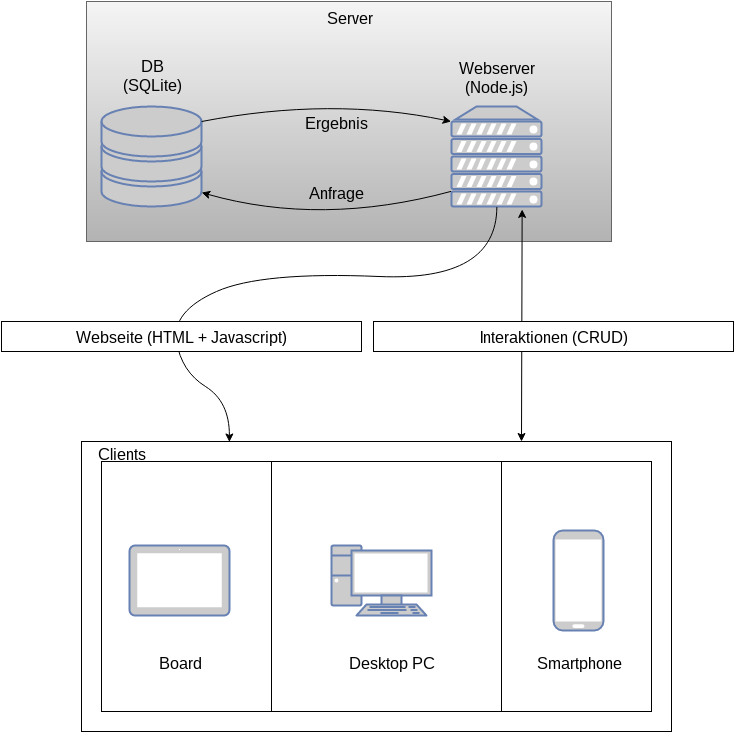
\includegraphics[width=0.8\textwidth]{./img/Systemaufbau.png}
  \caption{Bauhausboards - Systemaufbau}
  \label{img:Systemaufbau}
\end{figure}
\\
Da die Nutzer die Möglichkeit bekommen sollten, individuellen Inhalt präsentieren zu können, musste ein geeigneter Editor programmiert werden.
Damit sollte es möglich sein, einfache Zeichnungen anzufertigen, Texte zu schreiben oder Bilder hochladen zu können.
Es war wichtig, dass der Editor die Funktionen eines Whiteboards in manchen Zügen übernehmen oder möglicherweise sogar verbessern konnte.
\\
Folgende Whiteboard-Funktionen musste der Editor daher abbilden:
\begin{itemize}
  \item Zeichnen mit verschiedenfarbigen Stiften
  \item Entfernen von Zeichnungen mit einem Schwamm
  \item Anbringung von Bildern oder Ausdrücken per Magnet
  \item Neuanordnung von aufgehängten Elementen
\end{itemize}
Als Grundlage für den Editor entschied ich mich für die Javascript Bibliothek Paper.js\footurl{http://paperjs.org}{01.12.2015}.
Es ist ein Open Source Framework für die Darstellung und Manipulation von Vektorgrafiken, welches auch die Grundlage des Editors aus dem NetBoards Projekt bildete\cite{wood:2014}.
\\
\\
Eine weitere wichtige Entscheidung war, dass nur die an den Boards registrierten Nutzer den dargestellten Inhalt ändern können sollten, da sich in der Vorstudie herausstellte, dass es durch die Anonymität der Besucher häufig zu unerwünschten Änderungen kam.
Dadurch sollte ein Sicherheitsaspekt geschaffen werden, weil keine andere Person die Daten ändern durfte außer derjenige, der sie erstellt hat.
\\
Den Besuchern sollte jedoch weiterhin die Möglichkeit geboten werden, mit den registrierten Nutzern in Kontakt zu treten. Dies konnte mit einer separaten Nachrichtenfunktion realisiert werden.
\\
Zur Planung erstellte ich zu Beginn einen Paper-Prototype\footnote{Ein Paper-Prototype ist ein auf Papier gezeichneter Entwurf} für das Interface und die Funktionen, die es bieten sollte. Dieser Entwurf befindet sich im Anhang.










\subsection{Entwurf des Interfaces}\label{Entwurf des Interfaces}
\subsubsection{Hauptansicht}\label{Hauptansicht}
Da den Gästen in der Vorstudie nicht bewusst war, dass mehrere Personen auf dem Board registriert waren, was der Größe des Tablets zu verschulden war, musste der vorhandene Platz anders aufgeteilt werden. Das NetBoards System teilte den Bereich verschiedener Benutzer räumlich, indem es den verfügbaren Platz durch die Anzahl der registrierten Benutzer teilte.
Auf einem 10,1 Zoll großem Tablet macht dieser Ansatz jedoch wenig Sinn, da bei mehr als einem Benutzer der verfügbare Platz zu klein wäre \abb{img:aufteilungMainView}.
\begin{figure}[h!]
  \centering
    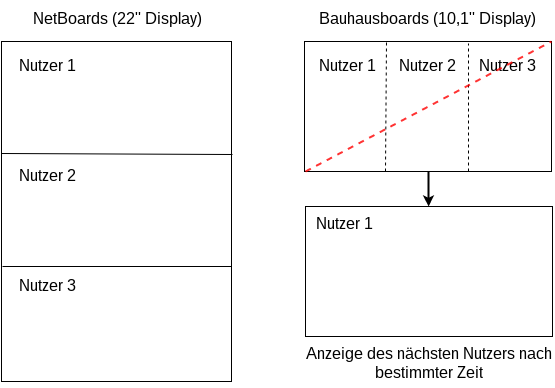
\includegraphics[width=0.68\textwidth]{./img/AufteilungMainView.png}
  \caption{Vergleich der Platzverteilung NetBoards - Bauhausboards}
  \label{img:aufteilungMainView}
\end{figure}
\\
Deswegen sollte jeder registrierte Nutzer die ganze Fläche zu Verfügung haben, wobei nach einer festgelegten Zeit die Sicht wechselt und die Daten des nächsten Nutzers angezeigt wird.
\\
Die Datenansicht sollte in zwei Schichten aufgeteilt werden. Zum einen eine Editor-Schicht für selbst gezeichnete Skizzen, Texte, Bilder und animierte Gifs sowie eine Hintergrundschicht, in der die Nutzer eine Webseite anzeigen lassen können. Da NetBoards diese Funktion bereits bot und die Testnutzer in der Vorstudie diese ebenfalls nutzten, entschied ich mich, sie auch umzusetzen.
\\
Um auf der Webseite navigieren zu können musste es dafür ein Menü geben, das auf den Tablets nicht viel Platz benötigte. Die beste Variante dafür war eine Sidebar, die standardmäßig eingeklappt ist und sich per Klick oder Swipe-Geste\footnote{Eine Swipe-Geste ist eine Fingergeste, bei der eine Aktion durch seitliches Wischen des Fingers auf dem Interface ausgeführt wird.} öffnen ließ.
In diesem Menü sollten alle Navigationselemente untergebracht sein. 
\\
Um Informationen über die Nutzer anzeigen zu können, wurde eine zusätzliche Fläche benötigt.
Dafür sollte im oberen Bereich des Displays ein Teil nur für solche Informationen reserviert sein. 
In diesem Header konnte man das Profilbild, den Namen und eine Beschreibung des aktuell ausgewählten Nutzers darstellen.
In der Vorstudie wurde es sehr gut aufgenommen, dass einer der Nutzer seinen aktuellen Status angegeben hat.
Deswegen sollte diese Funktion neben den Nutzerinformationen im Header zu finden sein.
\begin{figure}[h!]
  \centering
    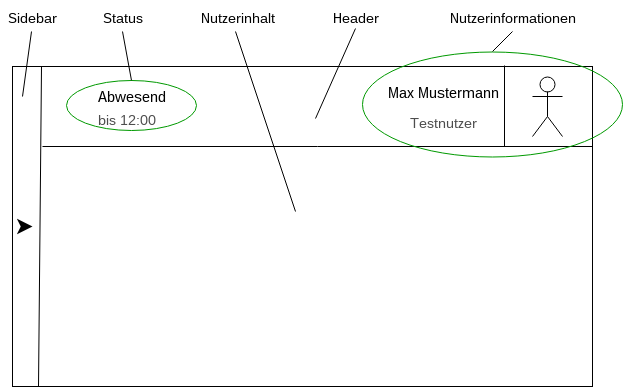
\includegraphics[width=0.7\textwidth]{./img/MainViewAufbau.png}
  \caption{Aufbau der Hauptansicht}
  \label{img:mainView}
\end{figure}
\\
%Messages
% \todotext{können,können,können ... -> ändern}\\
Damit die Gäste mit den Besitzern in Kontakt treten können, musste es eine Nachrichtenfunktion geben.
Dabei sollten die Benutzer, die eine Nachricht erstellen wollen, einen oder mehrere Besitzer auswählen dürfen.
Danach soll der Editor aktiviert werden.
Die Besucher können eine Zeichnung oder einen Text erstellen.
Die Besitzer müssen, nachdem die Nachricht abgeschickt wurde, darüber informiert werden, dass ihnen eine Nachricht hinterlassen wurde.

\subsubsection{Benutzer-Backend}\label{Benutzer-Backend}
Die Besitzer der Boards sollten ihren öffentlichen Inhalt ändern, einen Status setzten und empfangene Nachrichten lesen können.
Dafür müssen sie sich vorher im Benutzer-Backend authentisieren.
\\
Das Backend soll den Nutzern die Möglichkeit bieten, ihre Nutzerdaten, wie das Profilbild, die Benutzerbeschreibung oder das Passwort ändern zu können.
\\
Um die angezeigten Daten der Hauptseite anzupassen, wird der selbe Editor verwendet, der auch bei der Erstellung von Besuchernachrichten zum Einsatz kommt.
\\
Für den Status sollen die Nutzer einen kurzen Text und den Endzeitpunkt festlegen, der dann auf der Hauptseite angezeigt wird.
\\
Außerdem mussten sie die Möglichkeit bekommen, erhaltenen Nachrichten einsehen zu können. Ungelesene Nachrichten mussten dabei besonders gekennzeichnet werden.\\
Die Änderung der Benutzerdaten sollten in einem gesonderten Einstellungsbereich möglich sein.
\\
Da das Benutzer-Backend auch vom aufgehängten Display aus erreichbar sein sollte, damit die Nutzer beim Verlassen des Raumes schnell einen Status setzen konnten, mussten sie sich schnell authentisieren können.
Deswegen entschied ich mich für zwei Authentisierungsmethoden.
Ein vierstelliger Pin sollte zur schnellen Anmeldung in das Backend dienen.
Die Benutzereinstellungen konnten dann nach einer klassischen Passwortauthentisierung vorgenommen werden.
% \\\todotext{Angeben bei den Routen: was macht der Doppelkreis}\\
\begin{figure}[h!]
  \centering
    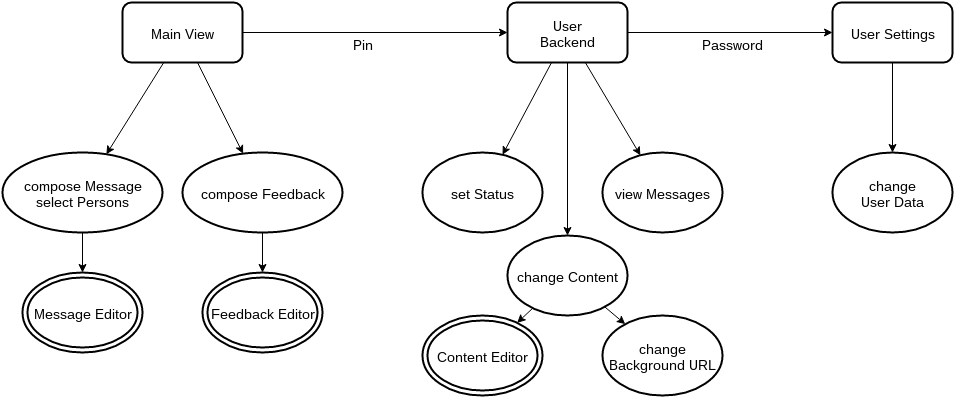
\includegraphics[width=0.9\textwidth]{./img/LocationsFrontend.png}
  \caption{Bauhausboards - Interface Funktionen mit Editorkomponenten}
  \label{img:Interface}
\end{figure}

\subsubsection{Administrator-Backend}\label{Administrator-Backend}
Der Administrator der Boards muss die Funktionen bekommen, das System verwalten zu können. Das beinhaltet das Erstellen, Ändern und Entfernen von Nutzern, sowie Board-Instanzen.
\\
Zudem soll er für Studienzwecke die Inhalte und Nachrichten der Benutzer einsehen können.

\subsection{Entwurf der Datenbank}\label{Entwurf der Datenbank}
Durch die geplanten Funktionen mussten anfallende Daten in einer Datenbank gespeichert werden.
Es bestand die Möglichkeit, eine dokumentenbasierte oder eine relationale Datenbank dafür zu nutzen.
Eine dokumentenbasierte Datenbank hätte den Vorteil gehabt, dass alle Anfragen eine JSON-Zeichenkette zurückgegeben hätten. JSON wird häufig in der Verbindung mit Javascript und dessen Serverkommunikation verwendet.
Relationale Datenbanken hingegen verwenden eine Tabellenstruktur für die Speicherung von Daten. Mit ihnen lassen sich Beziehungen zwischen den Daten einfacher darstellen.
\\
Für die Datenbank von Bauhausboards entschied ich mich für eine relationale Datenbank, weil die Einarbeitungszeit zu lang gedauert hätte, um mit dokumentenbasierten Datenbanken umgehen zu können.
% \\\todotext{ER Diagram zu groß}\\
\begin{figure}[h!]
  \centering
    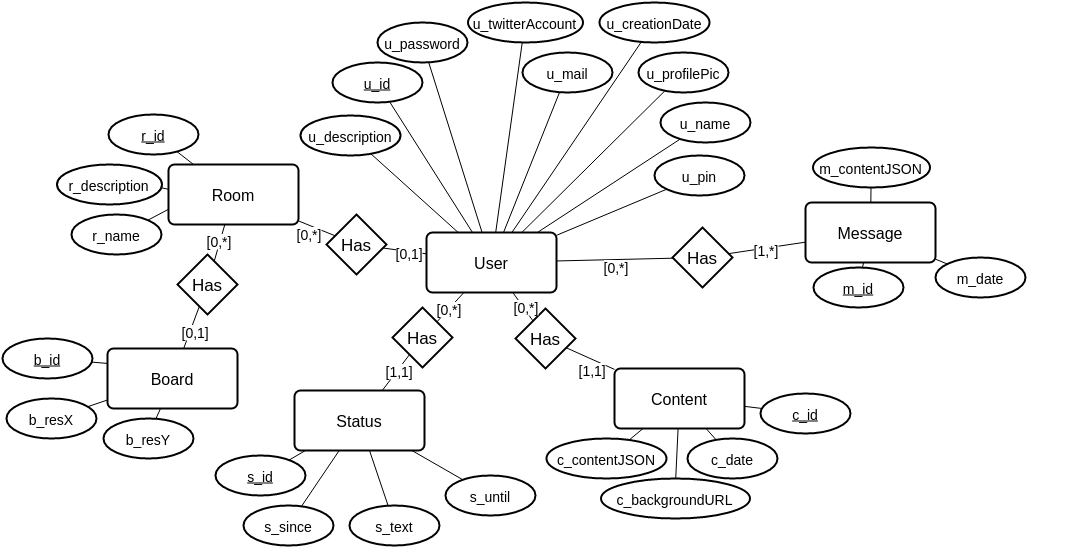
\includegraphics[width=1\textwidth]{./img/ER01.png}
  \caption{Bauhausboards - Entity Relationship Diagramm}
  \label{img:ER01}
\end{figure}
% \begin{figure}
%   \centering
%   \importsvg{ER01}
%   \caption{asdasd}
% \end{figure}
\\
Der Datenbankentwurf beinhaltete 6 Objektklassen, dargestellt als Tabellen. Um alle Objekte eindeutig beschreiben zu können, wurde in jeder Tabelle eine ID als Primärschlüssel\footnote{Ein Primärschlüssel ist ein Attribut zur eindeutigen Identifikation eines Datensatzes} hinzugefügt.
% \\\todotext{soll ich bei den Attributen noch auf die Datentypen eingehen?}\\
\subsubsection{User Tabelle}\label{User Tabelle}
Die User-Tabelle ist die Haupttabelle und dient zur Speicherung von Nutzeraccounts. Ein Nutzer muss auf jeden Fall einen Namen, eine Emailadresse, ein Passwort und einen Pin haben.
Zusätzlich können die Nutzer auch ein Profilbild, eine eigene Beschreibung und einen Twitter-Account angeben.
Wenn ein Benutzeraccount erstellt wird, soll das aktuelle Datum mitgespeichert werden.
\\
Ein Benutzer kann entweder in einem oder keinem Raum arbeiten. Er kann beliebig viele Status und Inhalte erzeugen und beliebig viele Nachrichten erhalten.
\subsubsection{Board Tabelle}\label{Board Tabelle}
Diese Tabelle ist die digitale Repräsentation von tatsächlich aufgehängten Displays. Da verschiedene Tablets eine unterschiedliche Auflösung haben können, musste diese in der Datenbank für jedes Board gespeichert werden. Ein Board kann entweder noch keinem oder genau einem Raum zugeordnet sein.
\subsubsection{Room Tabelle}\label{Room Tabelle}
In dieser Tabelle werden die möglichen Räume, vor denen Boards angebracht werden können, registriert. Jeder Raum hat einen Namen und möglicherweise eine Beschreibung. Ein Raum kann entweder keinem oder mehreren Boards zugeordnet sein. Zudem können beliebig viele Personen in einem Raum arbeiten.
\subsubsection{Content Tabelle}\label{Content Tabelle}
Mit dieser Tabelle werden die Inhalte der Nutzer gespeichert. Ein Inhalt besteht aus einem JSON-Objekt und einem Erstelldatum. Wenn für den Inhalt eine Hintergrundwebseite angegeben wurde, wird deren Adresse ebenfalls an dieser Stelle eingetragen. Jeder Inhalt hat genau einen Nutzer, der ihn erstellt hat.
\subsubsection{Status Tabelle}\label{Status Tabelle}
Die Status Tabelle dient zur Speicherung von Nutzerstatus. Jeder Nutzerstatus hat einen Statustext, ein Erstelldatum, einen Endzeitpunkt und genau einen Ersteller.
\subsubsection{Message Tabelle}\label{Message Tabelle}
In der Message Tabelle werden Nachrichten abgelegt, die von Besuchern erstellt wurden. Eine Nachricht hat einen Nachrichteninhalt und ein Erstelldatum. Da die Nachricht an mehrere Besitzer adressiert sein kann, hat jede mindestens einen Empfänger.
\\
\\
Die Relationen zwischen User und Message, sowie zwischen User und Room müssen jeweils über eine dritte Tabelle dargestellt werden.
In diesen Tabellen sind dann nur die Primärschlüssel der beiden beteiligten Objekte gespeichert.






















\section{Umsetzung}\label{Umsetzung}
Die im Entwurf geplanten Konzepte wurden dann in ein lauffähiges System umgesetzt \abb{img:finalHauptseite}. Dabei änderten sich einige Ansätze und andere kamen neu hinzu.
\begin{figure}[h!]
  \centering
    \frame{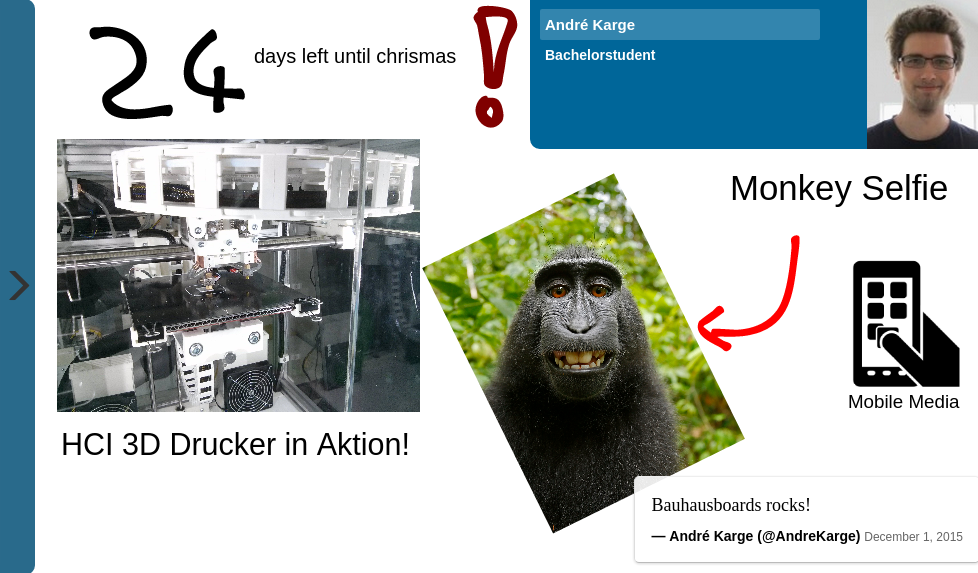
\includegraphics[width=1\textwidth]{./img/Hauptseite.png}}
  \caption{Bauhausboards - Hauptseite}
  \label{img:finalHauptseite}
\end{figure}

\subsection{Funktionen}\label{Funktionen}
Nachdem der Aufbau des Systems geplant war, mussten diese Pläne in ein lauffähiges Programm umgesetzt werden.
Um die Entwicklung mit Node.js zu vereinfachen, wurde das Framework Express\footurl{http://expressjs.com}{02.12.2015} verwendet. Damit ließ sich eine einfache Webapplikation erstellen.
\\
Da die hauptsächlichen Funktionen auf den Clients ausgeführt werden sollten, mussten diese in Javascript geschrieben werden.
Am wichtigsten war, dass sich die Seite nicht neu lud, wenn man durch sie navigierte. Dies wurde mit jQuery\footurl{https://jquery.com}{10.12.2015} realisiert. jQuery ist eine Bibliothek zur einfachen Manipulation der HTML-Struktur einer Webseite. Mit ihr war es einfach, die dargestellte Ansicht anzupassen.
\\
Falls an einer Stelle der Seite Daten vom Server benötigt wurden oder Daten auf dem Server geändert werden mussten, wurde dies mit Ajax-Anfragen durchgeführt. Ajax (Asynchronous Javascript and XML) ist eine Funktion für asynchronen Datenaustausch zwischen einem Client und einem Server.
Während ein Client auf die Ajax-Antwort des Servers wartet, können weiterhin andere Funktionen ausgeführt werden.
\\
% jquery touchswipe -> swipe tool für die swipe geste
Die Sidebar sollte keinen Platz wegnehmen und musste daher ein- und ausklappbar sein. Zudem sollten die Benutzer direkt erkennen, dass es sich um eine Sidebar handelt, wodurch ein Pfeil als Kennzeichnung daran angebracht wurde \abb{img:sidebar}.
Damit sie auf Tablets leichter zu öffnen war, nutzte ich TouchSwipe\footurl{http://labs.rampinteractive.co.uk/touchSwipe}{05.12.2015}. Mit dieser Bibliothek konnten Swipe-Gesten zum Aufruf von Funktionen genutzt werden.
\begin{figure}[h!]
  \centering
    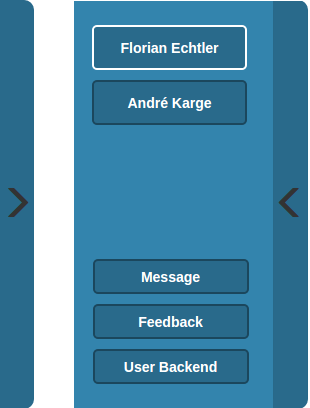
\includegraphics[width=0.4\textwidth]{./img/Sidebar.png}
  \caption{Bauhausboards - geschlossene und offene Sidebar}
  \label{img:sidebar}
\end{figure}
\\
% cryptoJS hash lib für passwort hashes
Die Passwörter und Pins durften nicht im Klartext gespeichert werden.
% \\\todotext{Nebensatz Hashes werden in DB gespeichert}\\
Dafür wurde die crypto-js\footurl{https://code.google.com/p/crypto-js}{05.12.2015} Bibliothek verwendet, um die sicherheitsrelevanten Daten mit SHA256\footnote{SHA256 (Secure Hash Algorithm 256) ist eine Krypto-Hashfunktion} zu hashen und sie danach in der Datenbank zu speichern oder sie mit den Werten der Datenbank abzugleichen.
\\
% emailJS = mail tool
Damit die Besitzer der Boards benachrichtigt werden, wenn Gäste ihnen Nachrichten hinterlassen, musste der Server Emails verschicken können.
Die Bibliothek emailjs\footurl{https://travis-ci.org/eleith/emailjs}{05.12.2015} brachte diese Funktion mit. Zusätzlich benötigte der Server zum Verschicken von Emails einen eigenen Mailserver oder wenigstens einen Account an einem anderen Mailserver.
In den Benachrichtigungsmails sollte ein Link mit einem Token\footnote{Ein Token ist ein Attribut zur Freigabe von Daten zwischen Parteien(Wer den Token hat, kann die Datei lesen)} zu der jeweiligen erhaltenen Nachricht im System sein. Der Token wurde mit crypto-js beim Abspeichern der Nachricht auf dem Server erzeugt. Wenn der Empfänger auf den Link klickt, wird der Token geprüft und die entsprechende Nachricht angezeigt. Dafür muss er sich nicht extra authentisieren.
\\
Die Farbgestaltung der Seite wurde schlicht gehalten und orientierte sich an den Hausfarben der Medienfakultät der BUW.
\\
Während der Umsetzung änderte sich die Entscheidung, alle Funktionen in einer einzigen Seite anzubieten, vom geplanten Konzept.
\\
Es war ursprünglich geplant, dass der Administrator normal über die Seite die Administratorfunktionen ausführen kann. Da diese Funktionen aber rein funktional waren und nicht auf den Boards gebraucht wurden, ergab es mehr Sinn diese gesondert in eine zusätzlichen Webseite auszulagern.
\\
\\
Zur geplanten Statusfunktion kam während der Umsetzung noch die Idee auf, dass sich Nutzer als ``Abwesend'' markieren konnten. Dazu sollte im Benutzer-Backend eine zusätzliche Option eingebaut werden. Um diesen Status zu kennzeichnen, wurden dabei die Profilbilder der Nutzer ausgegraut und ein Text darüber angezeigt, dass der Nutzer zur Zeit nicht verfügbar ist (Abb. \ref{img:UserAvailable}).
% \todotext{Bilder vergleich Anwesend / nicht anwesend}\\
\begin{figure}
  \centering
    \subfigure[Nutzer verfügbar]{
      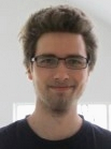
\includegraphics[width=0.28\textwidth]{./img/UserAvailable.png}
      % \label{img:UserAvailable}
    }
    \subfigure[Nutzer nicht verfügbar]{
      
\includegraphics[width=0.28\textwidth]{./img/UserUnavailable.png}
      % \label{img:UserUnavailable}
    }
  \caption{Bauhausboards - Nutzerstatus}
  \label{img:UserAvailable}
\end{figure}
Außerdem kam eine Twitter-Funktion hinzu. Die Besitzer der Boards konnten einen Twitteraccount in ihren Einstellungen eintragen, wodurch auf ihrer Seite ihr aktuellster Tweet geladen und angezeigt wurde \abb{img:twitter}. 
% \\\todotext{twitter Bild}
\begin{figure}
  \centering
    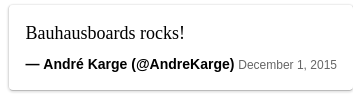
\includegraphics[width=0.4\textwidth]{./img/TwitterFeature.png}
  \caption{Bauhausboards - Twitterfunktion}
  \label{img:twitter}
\end{figure}

%%%%%%%%%%%%%%%%%%%%%%%%%%%%%%%%%%%%%%%%%%%%%%%%%%%%%%%%%%%%%%%%%%%%%%%%%%%%%%%%

\subsection{Editor}\label{Editor}
Der Kern der Client-Funktionen war der Editor zum Erzeugen von Nutzer-Inhalten und Besuchernachrichten. Da Paper.js nur ein Framework war, musste das Interface dafür von Grund auf implementiert werden.
Voraussetzungen für Paper.js war, dass die Webseite mit dem neuesten HTML5 Standard entwickelt wurde, weil diese Version ein neues Canvas-Element bot, mit dem Grafiken gezeichnet werden konnten.
\\
Die Funktionen des Editors erfüllten die Anforderungen des Entwurfs sehr gut.
Mit einer Stiftfunktion ist es möglich, Zeichnungen per Hand anzufertigen. Dabei kann der Benutzer die Linien in vier verschiedenen Linienstärken zeichnen.
\\
Außerdem wurde ein Textwerkzeug implementiert, mit dem ein Text per Tastatur eingegeben werden konnte \abb{img:editorTextSketch}.
\begin{figure}
  \centering
    \frame{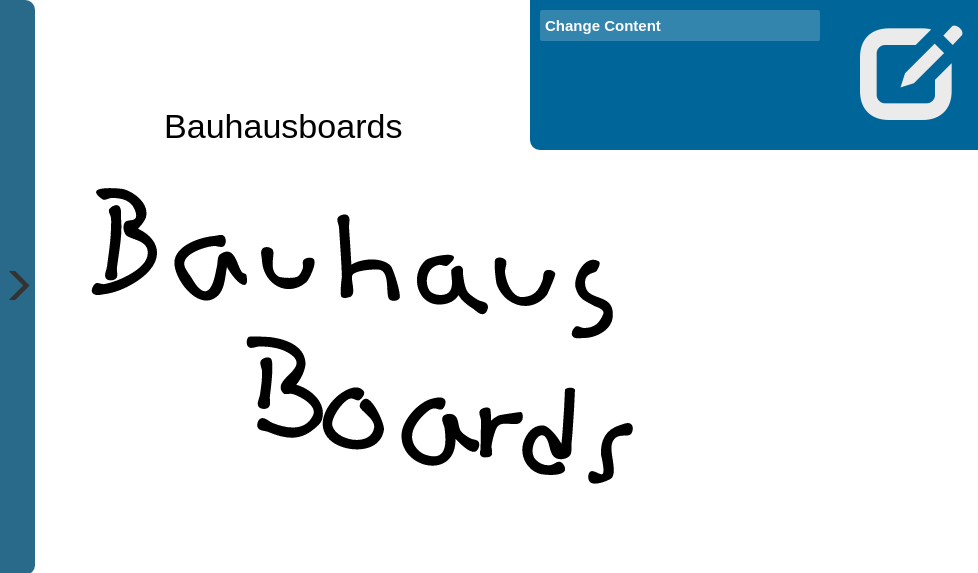
\includegraphics[width=0.85\textwidth]{./img/EditorTextAndSketch.png}}
  \caption{Bauhausboards - Text Sketch}
  \label{img:editorTextSketch}
\end{figure}
\\
Damit das Gezeichnete beliebig auf der Zeichenfläche angeordnet werden kann, musste es ein Auswahlwerkzeug geben \abb{img:editorObjectSelection}.
Die Nutzer konnten damit einen Auswahlrahmen um Objekte ziehen, welche dadurch markiert wurden.
Die Markierung zeichnete sich durch ein Auswahlrechteck mit Kreisen an den Ecken, in der oberen Mitte sowie einem kleinen Menü aus.
%, dass um die markierten Objekte ein Auswahlrechteck mit Kreisen an den Ecken und der oberen Mitte, sowie einem kleinen Menü erschien.
Durch Ziehen des Auswahlrechteckes wurde die Auswahl an eine gewünschte Stelle verschoben.
Zudem war es möglich, die Auswahl durch Klick auf die Kreise in den Ecken des Auswahlrechteckes zu skalieren oder durch Klick auf den Kreis in der oberen Mitte zu rotieren.
Die Funktionen des kleinen Menüs beinhalteten das Löschen oder Kopieren der Auswahl, sowie das Platzieren vor oder hinter anderen Objekten auf der Zeichenfläche.
\begin{figure}
  \centering
    \frame{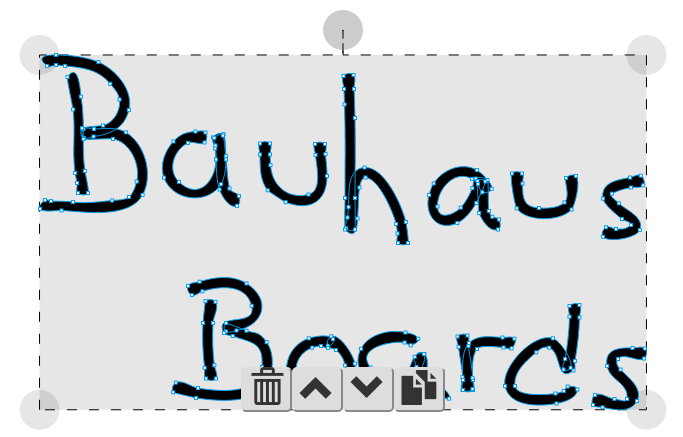
\includegraphics[width=0.8\textwidth]{./img/EditorObjectSelection.png}}
  \caption{Bauhausboards - Objekt Selektion}
  \label{img:editorObjectSelection}
\end{figure}
\\
Da es für Whiteboards und Tafeln Stifte oder Kreide in unterschiedlichen Farben gibt, musste es für den Editor eine Farbpalette geben, mit der man die Farbe der Zeichnungen und Texte ändern konnte.
\\
Die Funktion eines Tafelschwamms wurde mit einem einfachen Radiergummi-Werkzeug implementiert.
\\
Wie in jedem Editor, musste es eine Möglichkeit geben, die letzte Interaktion rückgängig zu machen oder wiederherzustellen. Dafür wurden Undo- und Redo-Funktionen eingebaut.
\\
Um Bilder darzustellen, konnten diese von einem anderen Browserfenster oder einem Dateibrowser per Drag-and-Drop in den Editor geschoben werden, wodurch diese auf den Server geladen und im Editor angezeigt wurden.
Damit war es auch möglich animierte Gifs hochzuladen.
\\
\\
Da man mit dem Editor alle Objekte verschieben, skalieren und rotieren konnte, hatte er einen Vorteil gegenüber klassischen Whiteboards und Tafeln.
Dort war es bisher nur möglich, per Magnet angebrachte Papiere zu verschieben oder zu rotieren.
Der Editor hatte durch die Skalierung von Objekten deswegen einen Freiheitsgrad mehr.
Zeichnungen konnten nur entfernt und an anderer Stelle wieder neu gezeichnet werden, welche in der digitalen Variante nur verschoben werden brauchten. Außerdem konnte man am Editor nachträglich die Farbe von Zeichnungen ändern, was am Whiteboard nicht möglich ist.
\\
Den größten Vorteil hat der Editor durch die Möglichkeit, animierte Gifs anzeigen zu lassen, da Whiteboards und Tafeln nur statischen Inhalt präsentieren können.
% \todotext{High Level View (wo laufen welche bibliotheken?)}\\
\begin{figure}[h!]
  \centering
    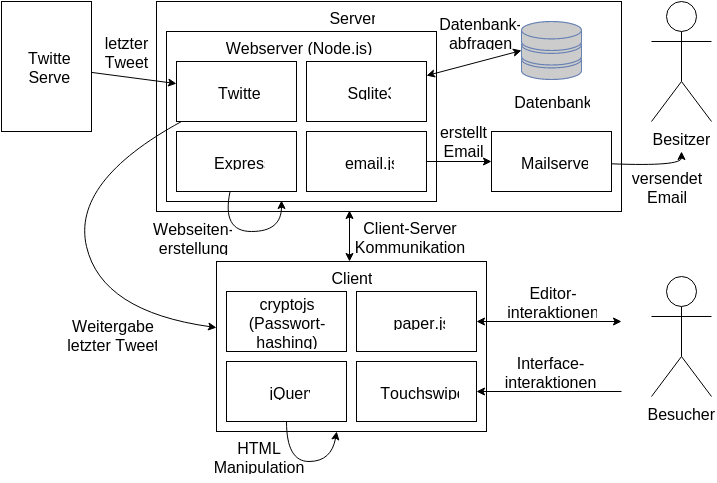
\includegraphics[width=0.75\textwidth]{./img/HighLevelSystemDiagram.png}
  \caption{Bauhausboards - Aufteilung der Systembibliotheken}
  \label{img:highLevelSystemDiagram}
\end{figure}

%%%%%%%%%%%%%%%%%%%%%%%%%%%%%%%%%%%%%%%%%%%%%%%%%%%%%%%%%%%%%%%%%%%%%%%%%%%%%%%%
\subsection{Probleme}\label{Probleme}
Während der Arbeit an Bauhausboards kamen diverse Probleme auf.
\\
% Editor
%- Gif Layer Hack
  % gif:
  % canvas element konnte nativ keine gifs anzeigen
  %  -> lösung: gif layer
%- Scale Problem ???
Da das HTML5 Canvas Element nur statischen Inhalt anzeigen konnte, musste die Anzeige von animierten Gifs auf andere Art gelöst werden.
Dazu wurde eine Gif-Schicht über den Editor gelegt.
Wenn sich ein Gif-Objekt in der Editor-Schicht befand, wurde dieses Objekt in die Gif-Schicht geladen und die Transformationen aus dem Editor auf die Kopie angewandt.
\\
%Problem Header
%- durch horizontale ausrichtung der tablets ist der Platz des header zu groß und wird verschwendet
%- wenn nur userimage, username, status, description usw angezeigt werden muss
%- Lösung: absolutes header div, welches oben rechts in der ecke ist
%  # content hat dadurch tatsächlich die größe des tablets
%  # platz wird nicht so stark verschwendet
Ein weiteres Problem war, dass durch die horizontale Ausrichtung der Tablets der Platz des Headers zu groß war, da er über die gesamte Breite des Tablets lief.
Weil er aber nur das Profilbild, den Namen, die Beschreibung und den Status eines angezeigten Nutzers beinhalten sollte, wurde er verkleinert.
Dadurch entstand mehr Platz für den Inhalt der Nutzer.
\\
%Problem: Desktop Version dimensions
%- die Auflösung auf dem Desktop ist größer als auf dem Tablet
%- content, der auf dem Desktop weiter rechts/weiter unten erstellt wird, verschwindet auf dem tablet :(
%- Lösungsansätze:
%  # Canvas resize auf größeren Auflösungen
%  # anzeige von linien, wie es auf dem tablet angezeigt wird
Hinzu kam das Problem, dass Desktop PC's eine größere Auflösung hatten als Tablets.
Deswegen konnten Zeichnungen, die außerhalb der Board-Auflösung erstellt wurden, nicht auf den Tablets angezeigt werden.
Die Lösung dafür war, die Größe des Editors auf die Auflösung des Tablets anzupassen und bei größeren Auflösungen diese Größe mit einem Rahmen zu kennzeichnen.
\\
%- Message Email mit image direkt in der NAchricht im HTML als <img> element ging nicht, da  cross origin resource sharing(CORS) nicht aktiviert ist (origin-clean flag false) deswegen geht die Funktion .toDataURL("image/png") nicht
%   * Zudem ist es schwer in der mail ein paperJS project in ein canvas einzubinden
%   * deswegen die Überlegung beim erstellen der message das canvas objekt direkt zu exportieren
% Das letzte Problem war, dass 


%%%%%%%%%%%%%%%%%%%%%%%%%%%%%%%%%%%%%%%%%%%%%%%%%%%%%%%%%%%%%%%%%%%%%%%%%%%%%%%%



















\section{Vergleich zu Hermes und NetBoards}\label{Vergleich zu Hermes und Netboards}
% \todotext{ist dieses Kapitel Notwendig?}\\
Im Vergleich zu NetBoards wurde bei Bauhausboards der Platz nicht durch die Anzahl der angemeldeten Benutzer geteilt.
Das hatte den Vorteil, dass jeder Benutzer die ganze Fläche zur Verfügung bekam.
Dadurch konnte jedoch immer nur ein Nutzer zur selben Zeit angezeigt werden.
\\
Bauhausboards bot, wie Hermes, die Funktion, den Besitzern der Boards Nachrichten zu hinterlassen, wohingegen NetBoards diese Funktion nicht hatte.
\\
Bei NetBoards kann jeder Gast den angezeigten Inhalt nach Belieben ändern.
Da sich in der Vorstudie von Bauhausboards gezeigt hatte, dass diese Funktion so nicht angebracht war, durften bei Bauhausboards nur die Besitzer diesen ändern und die Besucher in einer extra Funktion Nachrichten hinterlassen.
Wenn dann ein Besucher einem Besitzer eine Nachricht hinterlässt, wird dem Empfänger, wie beim Hermes System, eine Email geschickt.
\\
Der Editor von Bauhausboards basiert auf der gleichen Bibliothek, wie bei NetBoards. Zudem wurde die Idee zur Anzeige von Webseiten als Hintergrundschicht ebenfalls vom NetBoars System übernommen.
% \\\todotext{hier mehr?}
% Das Bauhausboards System übernimmt daher einige Ideen von früheren Projekten und